\documentclass{article}

\usepackage{amsmath}
\usepackage{amssymb}
\usepackage[T1]{fontenc}
\usepackage{enumitem}
\usepackage{lipsum}
					%oryginalnie 6 i 8
\usepackage[a4paper, total={6in, 9in}]{geometry}
\usepackage{amsthm}
% do bibliografii
\usepackage{hyperref}

%grafika
\usepackage{graphicx}
\graphicspath{ {./} }

%twierdzenia
\newtheorem{theorem}{Twierdzenie}[section]
\newtheorem{corollary}{Wniosek}[theorem]
\newtheorem{lemma}{Lemat}[theorem]
\newtheorem{theorem2}{Twierdzenie} %nieuzywane

%rysowanie
\usepackage{tikz}
%rysowanie grafow
\usetikzlibrary{shapes.geometric, arrows}
\tikzstyle{startstop} = [rectangle, rounded corners, minimum width=3cm, minimum height=1cm,text centered, draw=black, fill=red!30]
\tikzstyle{io} = [trapezium, trapezium left angle=70, trapezium right angle=110, minimum width=3cm, minimum height=1cm, text centered, draw=black, fill=blue!30]
\tikzstyle{decision} = [diamond, minimum width=3cm, minimum height=1cm, text centered, draw=black, fill=green!30]
\tikzstyle{process} = [rectangle, minimum width=3cm, minimum height=1cm, text centered, draw=black, fill=orange!30]
\tikzstyle{arrow} = [thick,->,>=stealth]

%geogebra
\usepackage{pgfplots}
\pgfplotsset{compat=1.15}
\usepackage{mathrsfs}
\usetikzlibrary{arrows}

\title{Laby}
\author{Patryk}



%tytul customowy

\begin{document}

% \maketitle
% \newpage

\begin{titlepage}
	\hfill \today

	\vspace{.2\textheight}

	\begin{center}
		{\LARGE\bfseries Title of the report\par}
		\vspace{3cm}
		Carl Capybara \par
		Walter Wombat \par
	\end{center}
	\vfill\centering  \par
\end{titlepage}

\tableofcontents
\newpage

\section{Laboratorium 8}
 
\begin{enumerate}[label=\underline{Przykład \arabic{enumi}}, wide=0pt]
	\item 
Niech $a$ i $b$  będą dowolnymi liczbami dodatnimi. Korzystając z indukcji matematycznej wykazać, że
\begin{equation*}
(a+b)^n <2^n(a^n+b^n),
\end{equation*}
dla dowolnego $n \in \mathbb{N} $


\item - cdots
Korzystając z zależności między średnimi wykazać, że dla dowolnej liczby naturalnej n prawdziwa jest nierówność:
$ \frac{1}{n+2} + 1\frac{1}{n+3}  + \frac{1}{n+4}  + ... + \frac{1}{3n+4}  \leq 1 $


\item - left, right
Wykaż, że:
\begin{enumerate}
	\item $\binom{30}{29} + \binom{31}{29} = \binom{32}{30} - \binom{5}{5}$
	\item 
		\begin{equation*}
			\sum_{k=0}^{3n} (-1)^k \binom{3n}{k} = 0
		\end{equation*}
\end{enumerate}


\item - mathbb, array
Niech $f : \mathbb{R} \to \mathbb{R} $ będzie funkcją daną wzorem:

\[ f(n) =
  \begin{cases}
    -x^2-6x-8 & \quad x \leqslant -3 \\
    x+2 & \quad x > -3
  \end{cases}
\]
Czy f jest bijekcją? W przypadku pozytywnej odpowiedzi wyznaczyć $f^{-1}$ 

\item - lim
	\begin{equation*}
		\lim\limits_{n \to \infty} - \frac{\sqrt[3]{5}+\sqrt{2}n^3}{3n^2+1} = -\infty
	\end{equation*}
	
\item - sum
	\begin{equation*}
		\displaystyle\sum_{n=0}^{\infty} \frac{\sin^2{n\pi}}{\ln{3n}}
	\end{equation*}
	
\item - int
	\begin{equation*}
		\int_{3}^{5} (x^2-5x+3)\cdot x \, dx
	\end{equation*}

\item - geq
	\begin{equation*}
		\forall \varepsilon > 0 \quad \exists n_0 \quad \forall n \geq n_0 \quad |a_n - 3| < \varepsilon
	\end{equation*}

\item - theorem
	\begin{theorem}
		Każdy ciąg {$x_n$} zbieżny w przestrzeni metrycznej (X,d) spełnia warunek Cauchy'ego.
	\end{theorem}
\item - tabular
	Utwórz tabelę
	
		\begin{tabular}{|l|c|c|}
		\hline
		x    & 0 & $\sqrt{3}$ \\ \hline
		f(x) & 3 & 5       \\ \hline
		\end{tabular}

\item - array
\[
  \begin{cases}
    -x^2-1 = y \\
    7y-3=2x
  \end{cases}
\]

\item - varepsilon
\begin{equation*}
	\textbf{L}^\varepsilon_t (x)\varphi (u,x,t) =
	\varepsilon^{-1}[E\{\varphi(u^\varepsilon_{n+1},
	x^\varepsilon_{n+1},
	\tau^\varepsilon_{n+1})|
	u^\varepsilon_n = u,
	x^\varepsilon_n = x,
	\tau^\varepsilon_n = t,\}]
\end{equation*}

\item - phi
\begin{equation*}
	p_{ij} = \prod_{c=1}^T k\left( \frac{\phi}{(|x_i-x_c|+|y_i-y_c|)^f} + 
	\frac{(1 -\phi)B^{g-f}}{(2B-|x_i-x_c|-|y_i-y_c|)^g}\right)
\end{equation*}

\item - cfrac
\begin{equation}
x = a_0 + \cfrac{123123123}{
	a_3 + \cfrac{4232}{
	a_3 + \cfrac{423232132}{
	a_39 + \cfrac{12322}{a_7}}}}
\end{equation}

\item - pmatrix
\[
	A_{m,n} = 	
	\begin{pmatrix}
	a_{1,1} & a_{1,2} & \cdots & a_{1,n} \\
	a_{2,1} & a_{2,2} & \cdots & a_{2,n} \\
	\vdots & \vdots & \ddots & \vdots \\
	a_{m,1} & a_{m,2} & \cdots & a_{m,n} 
	\end{pmatrix} 
\]

\item - langle, ...
	\[
		(a),
		[b],
		\{b\},
		|d|,
		\Vert e \Vert,
		\langle f \rangle,
		\lfloor g \rfloor,
		\lceil h \rceil,
		\ulcorner i \urcorner	
	\]

\item - binom

\begin{equation*}
	\sum_{i=1}^{[\frac{n}{2}]}
	\binom{x^{i^2}_{i,i+1}}{[\frac{i+3}{3}]}	
	\frac{
		\sqrt{\mu(i)^{\frac{3}{2}}(i^2-1)}}
		{\sqrt[3]{\rho(i)-2}+\sqrt[3]{\rho(i)-1}}
\end{equation*}

\item - align

\begin{equation}
\begin{aligned}[t]
    a_{11} & = b_{11} \\
    a_{21} & = b_{21} 
\end{aligned}
\qquad
\begin{aligned}[t]
    a_{12} & = b_{11}\\
    a_{22} & = b_{22}+c_{22}
\end{aligned}
\end{equation}

\item - dfrac
$$
	\Re z = \dfrac
	{n\pi \dfrac
			{\theta + \psi}
			{2}}
	{\left( \dfrac
			{\theta + \psi}
			{2}\right)^2 
		+ \left( \dfrac{1}{2}log
		  	\left| \dfrac{B}{A} \right|
		  \right)^2 
	}
$$

\item - underbrace
$$
	\underbrace{a_0 + a_1 + a_2 + \cdots + a_n}_x
$$

\end{enumerate}

\section{Laboratorium 9}
\subsection{cytowanie}
\lipsum*[10] \cite{Bhavani}
\lipsum*[10] \cite{Gumanski} %cytowanie

\subsection{twierdzenia, wnioski, tezy}

Twierdzenia mogą być łatwo definiowane:
\begin{theorem}
	Jeżeli $f$ jest funkcją dla której pochodna istnieje w każdym punkcie, wtedy $f$ jest funkcj
\end{theorem}

\begin{theorem}[Twierdzenie Pitagorasa]
\label{pythagorean}
	To jest twierdzenie o trójkątach i może być opisane przez równanie:
\[ a^2 +b^2 =c^2 \]
\end{theorem}

	Konsekwencją twierdzenia \ref{pythagorean} jest następujący wniosek.
	
\begin{corollary}
	Nie istnieje trójkąt prostokątny którego boki są długości 2cm, 3cm oraz 4cm.
\end{corollary}

	Jeżeli do twierdzenia nadałeś etykietę (komendą \textbf{label}) to możesz odwoływać się dyna
\begin{lemma}
	Dla danych dwóch odcinków o długościach $a$ oraz $b$ odpowiednio, istnieje liczba rzeczywist
\end{lemma}


\bibliographystyle{plain} %styl biblio
\bibliography{lab10literatura} % plik bib

\section{Laboratorium 10}

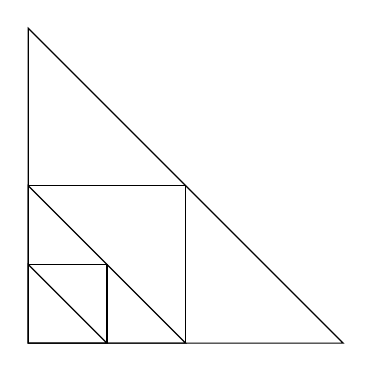
\begin{tikzpicture}
\draw (0,0) -- (4,0) -- (0,4) -- cycle;
\draw (2,0) -- (2,2) -- (0,2);
\draw (0,0) -- (2,0) -- (0,2) -- cycle;
\draw (1,0) -- (1,1) -- (0,1);
\draw (0,0) -- (1,0) -- (0,1) -- cycle;
\end{tikzpicture}

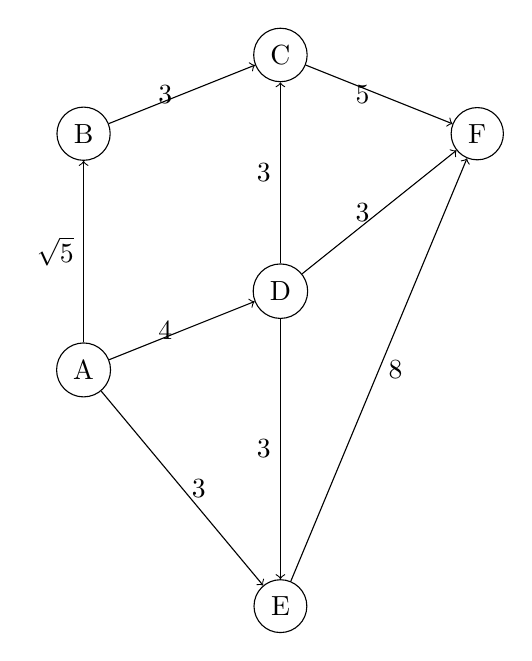
\begin{tikzpicture}
    \node[shape=circle,draw=black] (A) at (0,0) {A};
    \node[shape=circle,draw=black] (B) at (0,3) {B};
    \node[shape=circle,draw=black] (C) at (2.5,4) {C};
    \node[shape=circle,draw=black] (D) at (2.5,1) {D};
    \node[shape=circle,draw=black] (E) at (2.5,-3) {E};
    \node[shape=circle,draw=black] (F) at (5,3) {F} ;

    \path [->] (A) edge node[left] {$\sqrt{5}$} (B);
    \path [->](B) edge node[left] {$3$} (C);
    \path [->](A) edge node[left] {$4$} (D);
    \path [->](D) edge node[left] {$3$} (C);
    \path [->](A) edge node[right] {$3$} (E);
    \path [->](D) edge node[left] {$3$} (E);
    \path [->](D) edge node[left] {$3$} (F);
    \path [->](C) edge node[left] {$5$} (F);
    \path [->](E) edge node[right] {$8$} (F);   
\end{tikzpicture}

\url{https://www.overleaf.com/learn/latex/Inserting_Images}
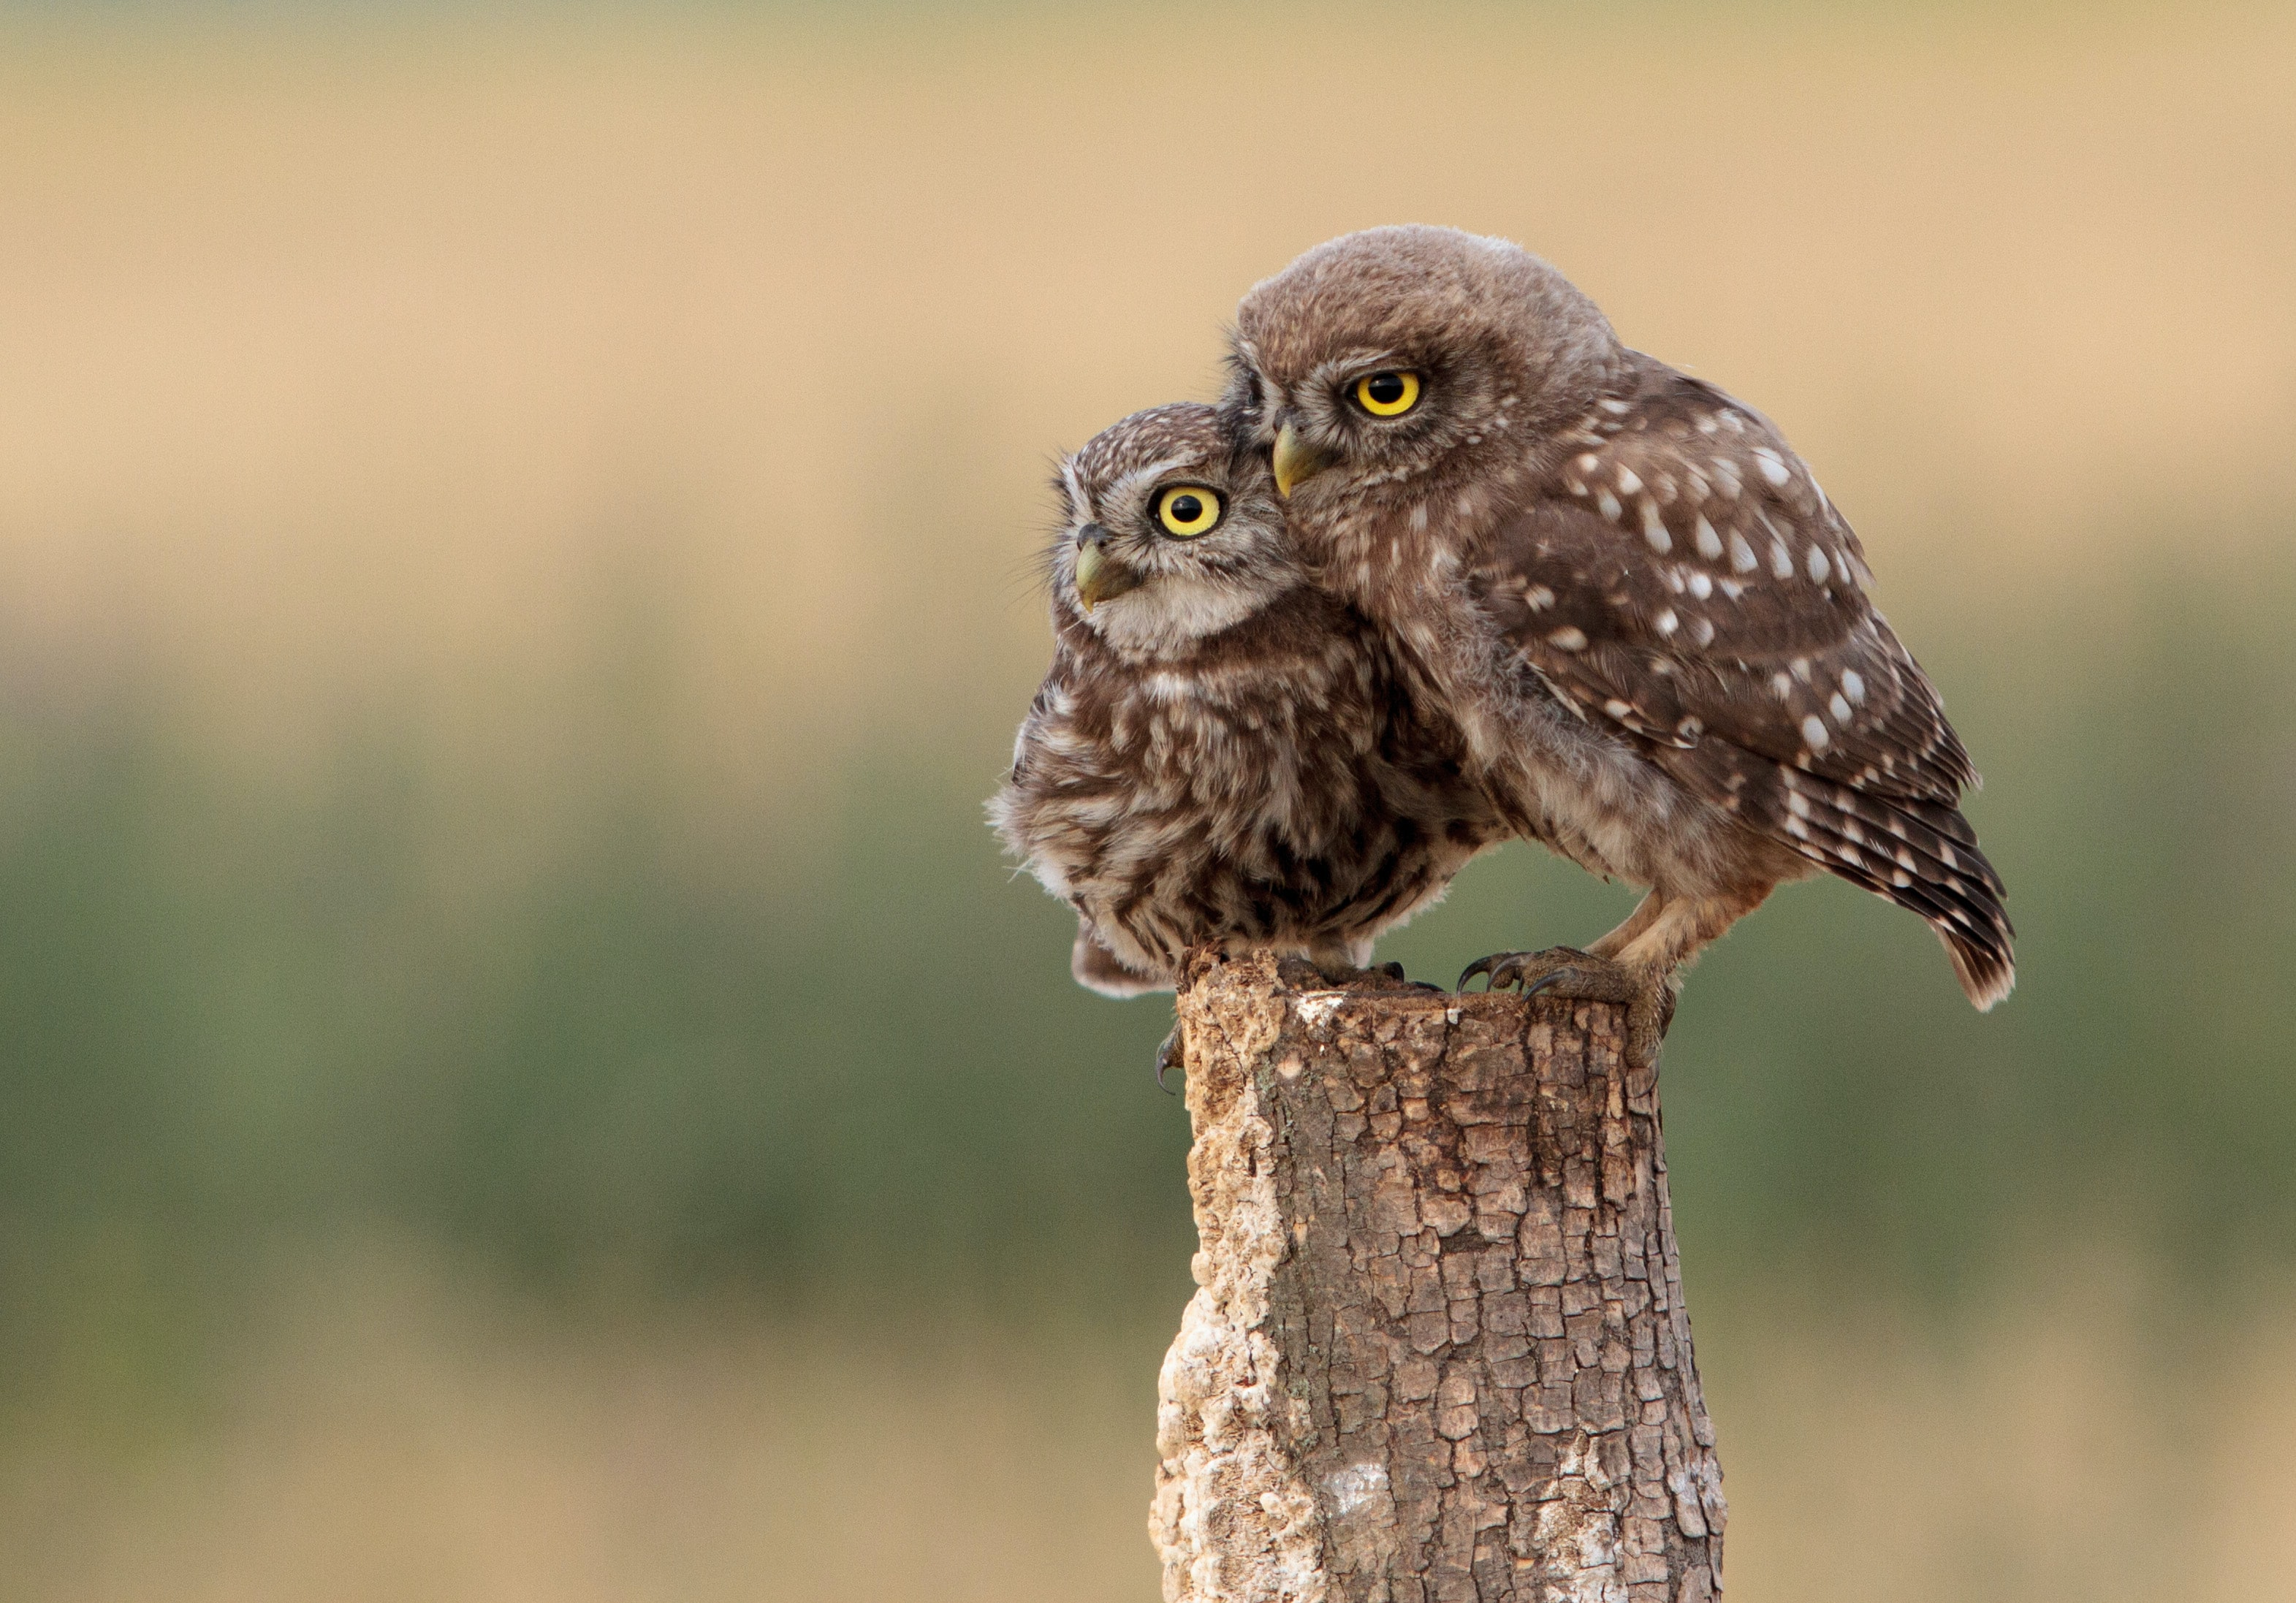
\includegraphics[scale=0.05]{img/sowa}
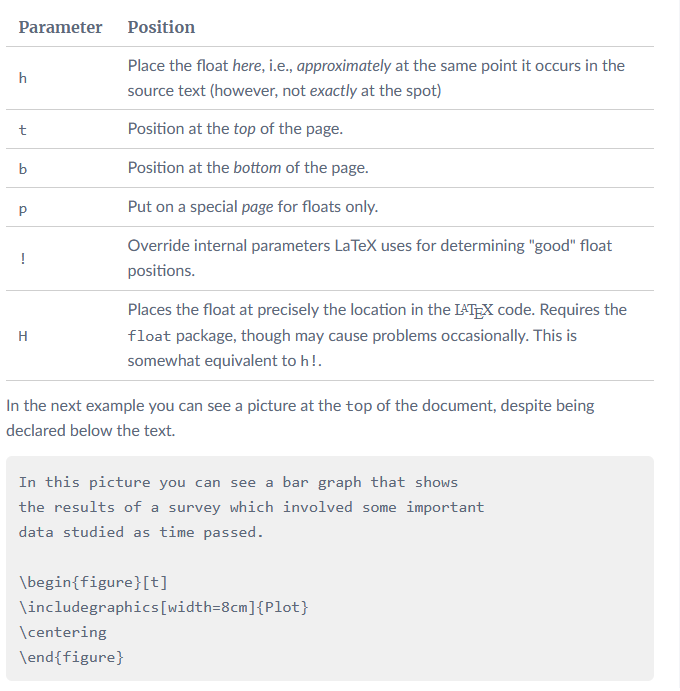
\includegraphics[scale=0.7]{pozycjonowanie}

\subsection{grafy}
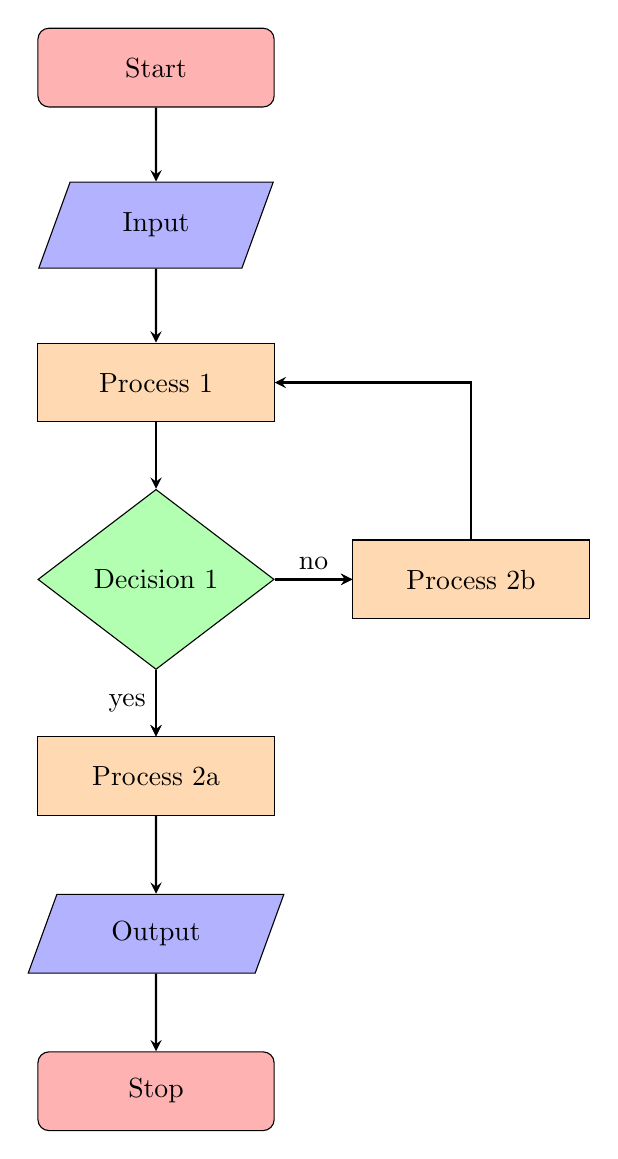
\begin{tikzpicture}[node distance=2cm]
\node (start) [startstop] {Start};
\node (in1) [io, below of=start] {Input};
\node (pro1) [process, below of=in1] {Process 1};
\node (dec1) [decision, below of=pro1, yshift=-0.5cm] {Decision 1};


\node (pro2a) [process, below of=dec1, yshift=-0.5cm] {Process 2a};
\node (pro2b) [process, right of=dec1, xshift=2cm] {Process 2b};
\node (out1) [io, below of=pro2a] {Output};
\node (stop) [startstop, below of=out1] {Stop};

\draw [arrow] (start) -- (in1);
\draw [arrow] (in1) -- (pro1);
\draw [arrow] (pro1) -- (dec1);
\draw [arrow] (dec1) -- (pro2a);
\draw [arrow] (dec1) -- (pro2b);

\draw [arrow] (dec1) -- node[anchor=east] {yes} (pro2a);
\draw [arrow] (dec1) -- node[anchor=south] {no} (pro2b);

\draw [arrow] (pro2b) |- (pro1);
\draw [arrow] (pro2a) -- (out1);
\draw [arrow] (out1) -- (stop);

\end{tikzpicture}

\section{Laboratorium 11}
\definecolor{xdxdff}{rgb}{0.49019607843137253,0.49019607843137253,1}
\definecolor{uuuuuu}{rgb}{0.26666666666666666,0.26666666666666666,0.26666666666666666}
\definecolor{zzttqq}{rgb}{0.6,0.2,0}
\definecolor{ududff}{rgb}{0.30196078431372547,0.30196078431372547,1}
\begin{tikzpicture}[line cap=round,line join=round,>=triangle 45,x=1cm,y=1cm]
\clip(-15.24,-8.12) rectangle (15.92,10.04);
\fill[line width=2pt,color=zzttqq,fill=zzttqq,fill opacity=0.10000000149011612] (-5.74,2.22) -- (-3.28,3.36) -- (-3.604022622414102,6.051878403673518) -- (-6.264279616189893,6.575550750725563) -- (-7.5843862347388455,4.2073196564986395) -- cycle;
\draw [line width=2pt,color=zzttqq] (-5.74,2.22)-- (-3.28,3.36);
\draw [line width=2pt,color=zzttqq] (-3.28,3.36)-- (-3.604022622414102,6.051878403673518);
\draw [line width=2pt,color=zzttqq] (-3.604022622414102,6.051878403673518)-- (-6.264279616189893,6.575550750725563);
\draw [line width=2pt,color=zzttqq] (-6.264279616189893,6.575550750725563)-- (-7.5843862347388455,4.2073196564986395);
\draw [line width=2pt,color=zzttqq] (-7.5843862347388455,4.2073196564986395)-- (-5.74,2.22);
\draw [line width=2pt] (-5.279051134624424,4.486510213910952) circle (1.8796737523967653cm);
\begin{scriptsize}
\draw [fill=ududff] (-5.74,2.22) circle (2.5pt);
\draw[color=ududff] (-5.58,2.65) node {$A$};
\draw [fill=ududff] (-3.28,3.36) circle (2.5pt);
\draw[color=ududff] (-3.12,3.79) node {$B$};
\draw [fill=uuuuuu] (-3.604022622414102,6.051878403673518) circle (2.5pt);
\draw[color=uuuuuu] (-3.44,6.49) node {$C$};
\draw [fill=uuuuuu] (-6.264279616189893,6.575550750725563) circle (2.5pt);
\draw[color=uuuuuu] (-6.1,7.01) node {$D$};
\draw [fill=uuuuuu] (-7.5843862347388455,4.2073196564986395) circle (2.5pt);
\draw[color=uuuuuu] (-7.42,4.63) node {$E$};
\draw [fill=xdxdff] (-6.877135333732006,5.4761062466495725) circle (2.5pt);
\draw[color=xdxdff] (-6.72,5.91) node {$F$};
\draw [fill=xdxdff] (-6.655084549879848,3.206000371875433) circle (2.5pt);
\draw[color=xdxdff] (-6.5,3.63) node {$G$};
\draw [fill=xdxdff] (-3.481904978515322,5.037363287816874) circle (2.5pt);
\draw[color=xdxdff] (-3.32,5.47) node {$H$};
\end{scriptsize}
\end{tikzpicture}

\section{Lab 12}
:c 


\end{document}
